\section{Experiment Evaluation}
\label{sec:experiment}
In this section, we first give some statistics of our dataset. Next, we evaluate the learned rules in both qualitative and quantitative aspects. Then, we compare our rule base with other existing causal knowledge bases. Next, we analyze and discuss some main steps for acquiring the rules. Finally, we showcase a small event graph instantiated from the rules. Our experiments are implemented in Python and SWI-Prolog and run on a computer with Intel Xeon 32 CPU (2.60GHz) and 173GB memory.

%related work ==> contribution 1
%contribution + analysis (weakness)
\begin{figure*}[!htbp]
	\centering
	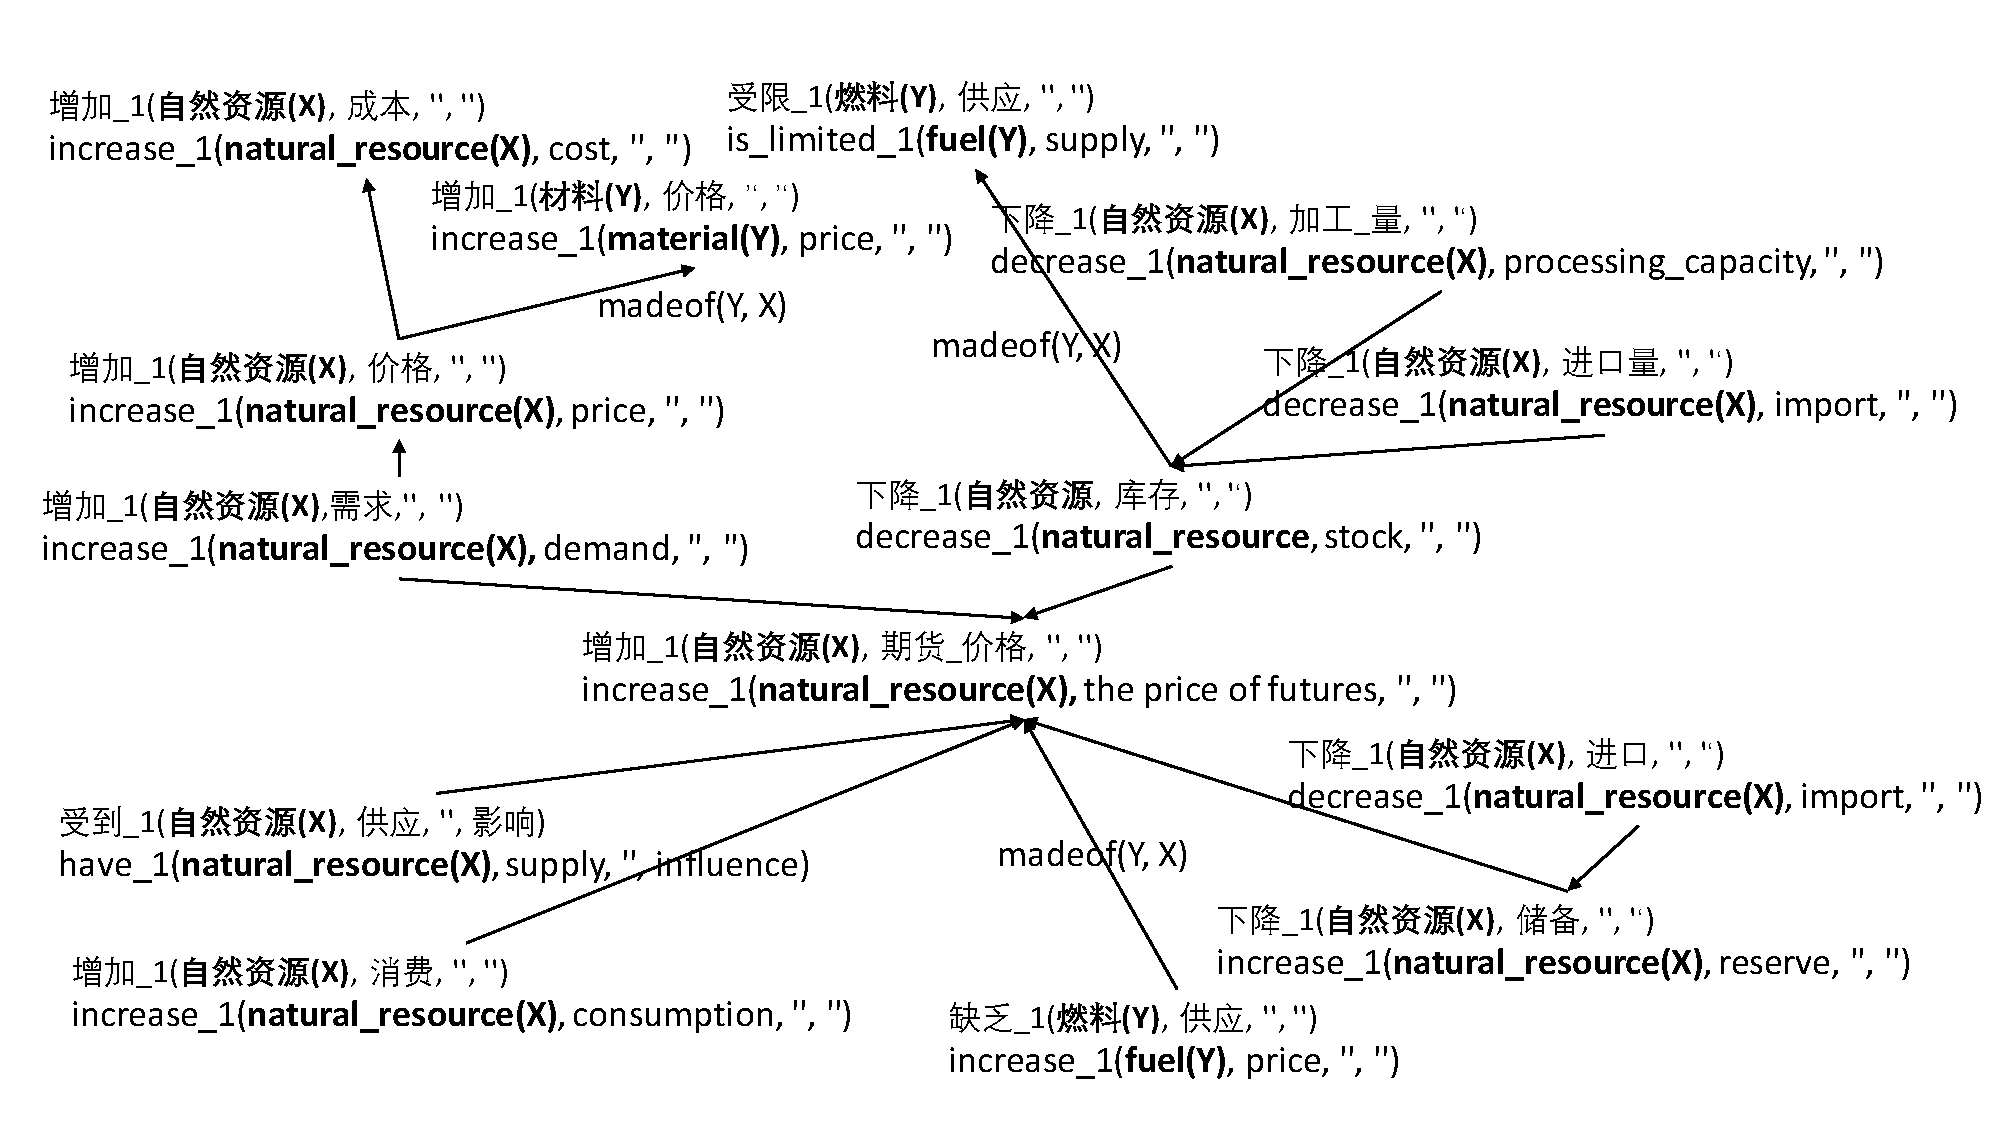
\includegraphics[width=0.95\linewidth]{figures/rule_graph}
	\caption{Examples of Good Rules}
	\label{fig:rule_graph}
\end{figure*}

\subsection{Dataset}
We crawled the text dataset from Sina Finance News,\footnote{\url{ http://finance.sina.com.cn}}, which is the largest financial news provider in China. The news data contains 4,991,000 articles, spanning from 2000/07/20 to 2017/12/31.
In these articles, there are \textbf{111,330,205} sentences in total. 
The number of unique sentences is \textbf{75,572,053}, accounting for \textbf{67.88\%} of the total sentences. 
The number of sentences with causal cue words such as ``因为'' is 7,147,141, accounting for 9.46\% of the total number of unique sentences and \textbf{14.20\%} (9.64\%/67.88\%) of the total sentences in online financial news.
%The news data containing 270,562 articles, from 2018/1/1 to 2018/11/2, is used to evaluate our framework. 
In the rule induction step of our rule learning framework, we set $\alpha$ to 0.5 to achieve an equal balance between generalization and specialization. 
We set $\gamma$ to 0.3 to control the Prolog engine to reason around two steps, since more than two steps lead to errors easily and explosive combination results\footnote{Some events can predict over 1,000 events within one step, as shown in Table \ref{tab:rule_conf}}, which makes the reasoning extremely slow.

%	\begin{table}[]
%		\caption{Dataset Information}
%		\begin{center}
%		\begin{tabular}{|l|l|l|}
%			\hline
%			Dataset       & Train & Test \\ \hline
%			Time Interval &       &      \\ \hline
%			Number        &       &      \\ \hline
%		\end{tabular}
%	\end{center}
%	\end{table}

\subsection{Rule Evaluation}
In this section, we evaluate these rules both quantitatively and qualitatively.
\paragraph{Quantitative Evaluation}
The number of the final rules we learned is \textbf{41,695}. All the rules will be graded as `good', `fair' or `bad'. The `good' means the rules are causally correct, `bad' means the rules are causally incorrect (e.g., an event should cause the price of corn to rise, but the rule indicates that its price will fall.) and `fair' means that the causality in the rule is vague and hard to tell its correctness. According to the ranking of rule confidence, we randomly select 100 rules from the top 10,000 rules and manually label them. In the first 10,000 rules, we can achieve the result shows that the ratios of `good', `fair' and `bad' are 65.0\%, 26.0\%, 9\%, respectively, and the result sampled from the whole rules is 46.0\%, 48.0\%, 6\%.

\paragraph{Qualitative Evaluation}
%\begin{align*}
%%	good
%%	{"c": ["过剩_1", "X_燃料", "产量", "", ""], "e": ["下降_1", "X_自然资源", "价格", "", ""], "relation": [["c_sc", "e_sc", "madeof"]], "ctx": {"senids": [1975666], "pattern_ids": [8]}, "ruleid": 5131, "confidence": 0.5657637042081998}
%&\text{1 (X, '产量/yield', '过剩/surplus', '', ''):-(Y, '价格/price', '下降/fall',} \nonumber\\
%&\text{'',''), IsA(X, '燃料/fuel'), IsA(Y, '自然资源/natural resource'),} \nonumber\\
%&\text{madeof(X, Y)} \\
%%{"c": ["结束_1", "X_国家", "罢工", "", ""], "e": ["下降_1", "X_金属", "价格", "", ""], "relation": [["e_sc", "c_sc", "atlocation"]], "ctx": {"senids": [341012], "pattern_ids": [6]}, "ruleid": 11607, "confidence": 0.5824045924950126}
%&\text{2 (X, '罢工/strike', '结束/stop', '', ''):-(Y, '价格/price', '下降/fall', }\nonumber\\
%&\text{'',''), IsA(X, '国家/nation'), IsA(Y, '金属/metal')}\nonumber\\
%&\text{, atlocation(Y, X)}	 \\
%%{"c": ["下降_1", "X_作物", "价格", "", ""], "e": ["减少_1", "", "", "X_作物", "面积"], "relation": [["c_sc", "e_oc", "=="]], "ctx": {"senids": [961411], "pattern_ids": [8]}, "ruleid": 978, "confidence": 0.5876590112986869}
%&\text{3 (X, '价格/price', '下降/fall', '', ''):-(X, '面积/area', '减少/fall', }\nonumber\\
%&\text{'',''), IsA(X, '作物/crop')} \\
%%fair
%%2{"c": ["下降_1", "X_国家", "储蓄率", "", ""], "e": ["下降_1", "X_国家", "增长率", "", ""], "relation": [["c_sc", "e_sc", "=="]], "ctx": {"senids": [1640122], "pattern_ids": [5]}, "ruleid": 213, "confidence": 0.7185889172176277}
%&\text{4 (X, '储蓄率/saving rate', '下降/fall', '', ''):-(X, '增长率/growth rate', }\nonumber\\
%&\text{'下降/fall','',''), IsA(X, '国家/nation')} \\
%%2{"c": ["下降_1", "", "X_产品", "", ""], "e": ["适合_1", "", "X_作物", "", ""], "relation": [["c_s", "e_s", "madeof"]], "ctx": {"senids": [1791763], "pattern_ids": [6]}, "ruleid": 19783, "confidence": 0.5634539402859007}
%&\text{5 ('', X, '下降/fall', '', ''):-('', Y, '适合/fit', '', ''), IsA(X, }\nonumber\\
%&\text{'产品/product'), IsA(Y, '作物/crop'), madeof(X, Y)}   \\
%%bad
%%1{"c": ["减少_1", "", "X_国家", "X_自然资源", "依赖性"], "e": ["增加_1", "", "", "X_燃料", "销量"], "relation": [["e_oc", "c_oc", "madeof"]], "ctx": {"senids": [1707156], "pattern_ids": [8]}, "ruleid": 4468, "confidence": 0.5717182258485046}
%%另一方面,由于日本、韩国和中国减少对中东地区进口原油的依赖性,道达尔公司希望增加对这三个国家的液化天然气销量。
%&\text{6 ('', X, '减少/fall', Y, '依赖性/dependence'):-('', '', '增加/increase',}\nonumber\\
%&\text{ Z,'销量/sales'), IsA(X, '国家/nation'), IsA(Y, '自然资源/natural-} \nonumber\\
%&\text{resource'), IsA(Z, '燃料/fuel'), madeof(Z,Y)}	
%\end{align*}
%Figure \ref{fig:rule_cases} shows some typical rules: 【1 and 2 are graded as `good', 3 and 4 are graded as `fair', and 5 and 6 are graded as `bad'.】

Figure \ref{fig:rule_graph} gives an overview of the good rules.
%These two good rules express the generalized and valuable knowledge.
%For example, rule 1 tells us that if the price of some natural resource rise, then the mining profit of the fuel, made of this natural resource, will increase. 
%Rule 2 tells us that if the price of some crop is low, then the sown area of this crop will decline.
\begin{figure}[htbp]
	\centering
	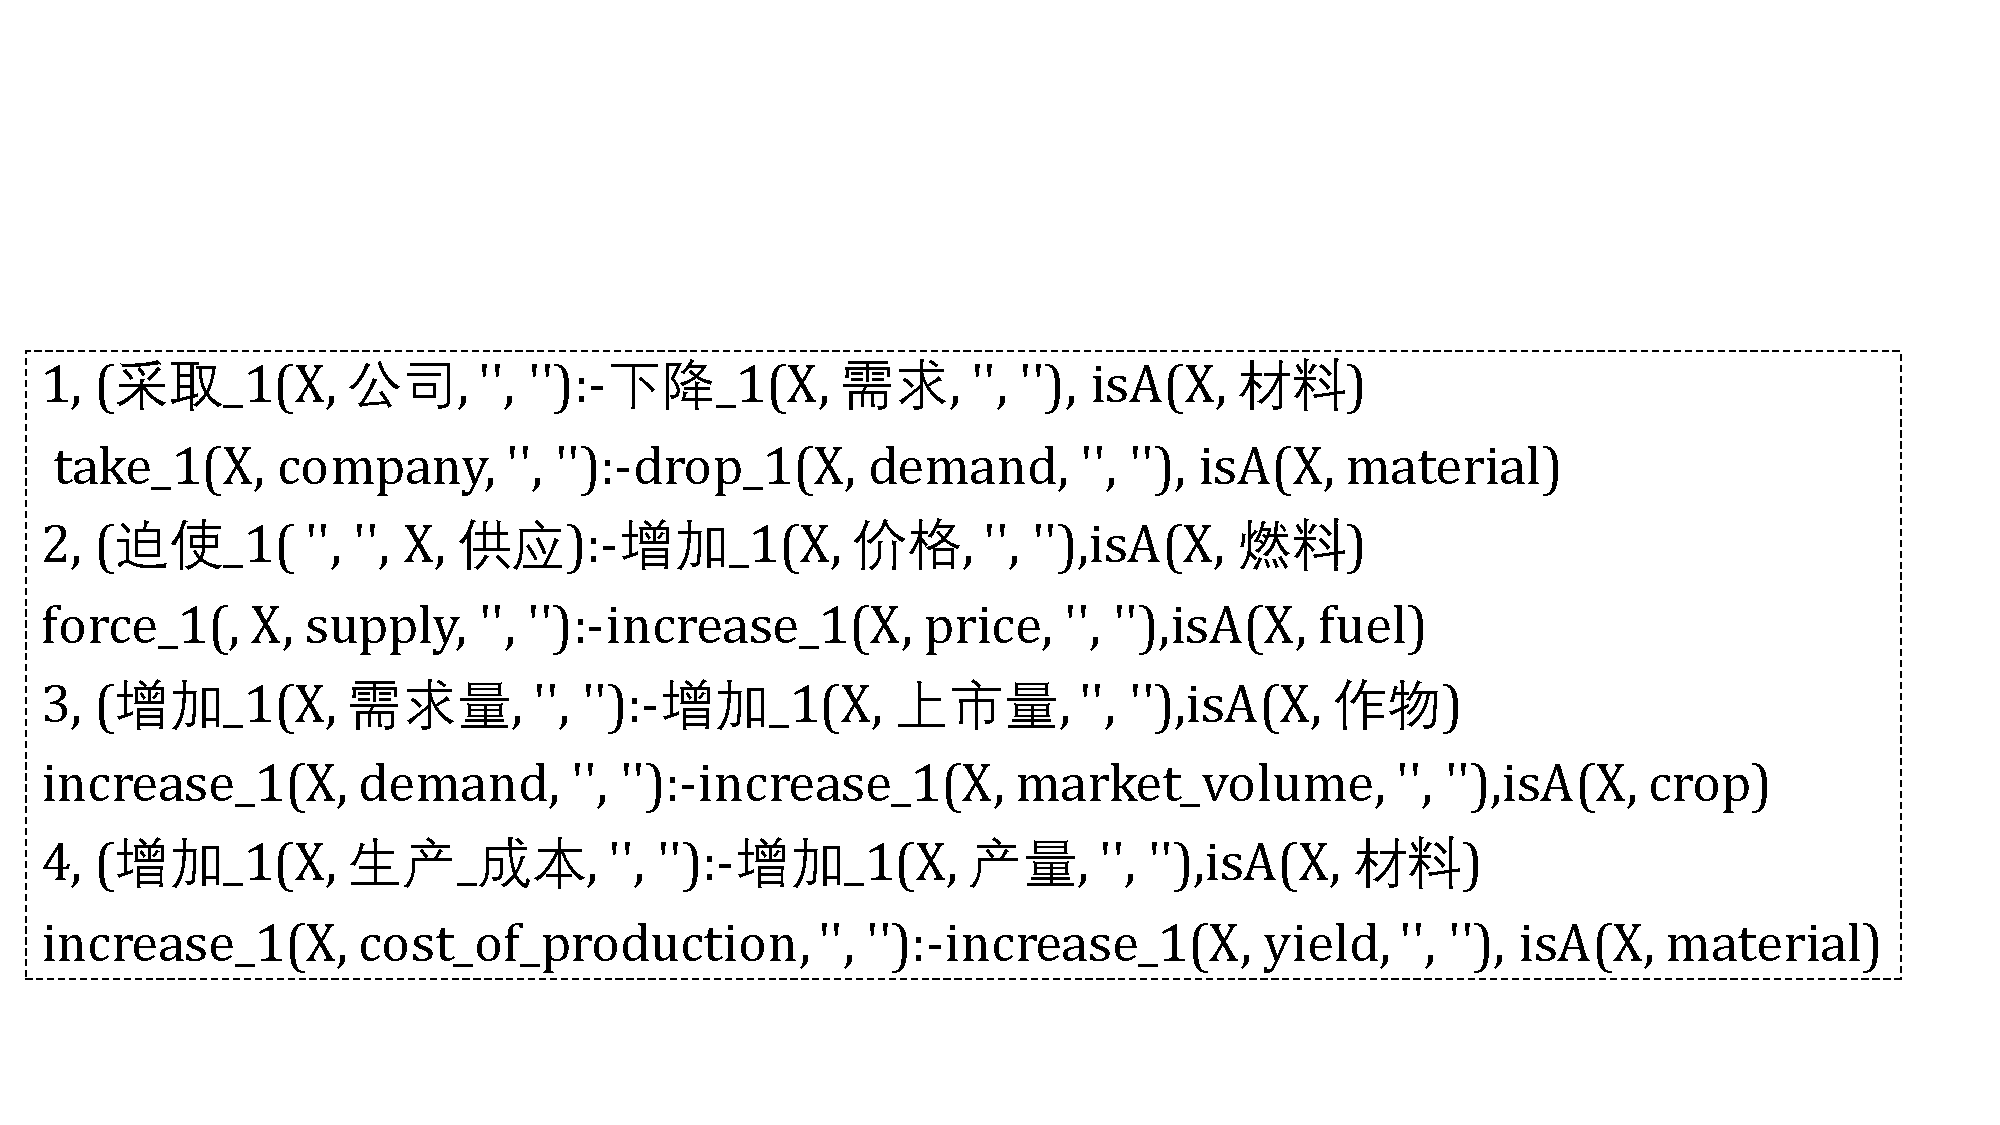
\includegraphics[width=0.95\columnwidth]{figures/rule_cases}
	\caption{Examples of Fair and Bad Rules}
	\label{fig:rule_cases}
\end{figure}
Figure \ref{fig:rule_cases} shows some typical `fair' and `bad' rules: 1 and 2 are graded as `fair'. 3 and 4 are graded as `bad'.
The flaws of these `fair' rules are as follows:
First, the events of cause or effect are incomplete. For example, both the effect events in 1 and 2 lack the objects, which makes the rules hard to understand. This problem is caused by the event extraction technique. The causal relations in both rule 3 and rule 4 are wrong.
For example, rule 3 means that if the yield of material increases, then the cost of its production will increase, which contradicts our common sense.
Some other problems also exist, such as weak causality captured by the loose causal patterns, verb disambiguation when normalizing predicates, noun disambiguation when generalizing rule instances.

\subsection{Comparison with existing resources}
We compare our rule base with other causal knowledge bases in various aspects in Table \ref{tab:comparison_rule_with_kbs}. 
It shows that our causal knowledge representation is more expressive because both concreteness and generality are good, which benefits from the fine-grained granularity of the concepts in our rules. 
Besides, our automatic knowledge acquisition is efficient.
The probabilistic feature, used to express the uncertainty of causal knowledge, is also effective, demonstrated in Section \ref{sec:end-to-end_rule}. 
Our rules can be directly used in Prolog to do reasoning, as shown in Section \ref{sec:executable_example}.
Moreover, our rule learning framework is easy to extend to the open domain.
\begin{table*}[htbp]
\caption{Comparison with existing knowledge bases}
\label{tab:comparison_rule_with_kbs}
\centering
\begin{tabular}{|c|c|c|c|c|c|c|c|c|}\hline
\textbf{Name}&\textbf{Number}&\textbf{Domain}&\textbf{Data/Structured}&\textbf{Concreteness}&\textbf{Generality}&\textbf{Source}&\textbf{Uncertainty}&\textbf{Accuracy}\\ \hline
CausalNet&\textbf{62,675,002}&\textbf{Open}&word/\textbf{Yes}&\textbf{good}&bad&\textbf{automatic}&No&-\\
\multicolumn{9}{|c|}{(drink, accident,36)}\\\hline
ConceptNet &89,416&\textbf{Open}&short text/No&\textbf{good}&bad&crowdsource&No&\textbf{100\%}\\
\multicolumn{9}{|c|}{(smoking, /r/Causes, cancer)}\\\hline
FrameNet&59&\textbf{Open}&frame/\textbf{Yes}&fair&\textbf{good}&crowdsource&No&\textbf{100\%}\\
\multicolumn{9}{|c|}{Killing(Killer, Place, Means, Victim, Instrument), CausativeOf, Death(Protagonist, Place, Manner, Time)}\\\hline
BECauSE 2.0 &1,803&\textbf{Open}&text/No&\textbf{good}&bad&crowdsource&No&\textbf{100\%}\\
\multicolumn{9}{|c|}{(we don’t have much time, so let’s move quickly.)}\\\hline
ATOMIC&568,312&\textbf{Open}&\textbf{logic event}/No&\textbf{good}&fair&crowdsource&No&86.2\%\\
\multicolumn{9}{|c|}{If ``PersonX pays PersonY a compliment", Then ``PersonY will smile"}\\\hline
Ours&42,037&Finance&\textbf{logic event}/\textbf{Yes}&\textbf{good}&\textbf{good}&\textbf{automatic}&\textbf{Yes}&65\%$^{\mathrm{a}}$\\ 
\multicolumn{9}{|c|}{
	\begin{tabular}{c}
		rise(Z, price, `', `'):-suffer(`', X, Y, attack), isA(X, country), isA(Y, disaster), isA(Z, metal), atLocation(Z, X) conf:0.842\end{tabular}}\\\hline
\multicolumn{9}{l}{$^{\mathrm{a}}$This is the ratio of ``good'' grade of top 10,000 rules.}
\end{tabular}
\end{table*}

%			Deductive Rule Instance&\TD{??}\\ 
%	\multicolumn{8}{|c|}{See above rule example in Figure\ref{fig:rules_case}}\\\hline

%	\multicolumn{8}{|c|}{
%		\begin{tabular}{c}
%			rise(Z,price,`',`'):-suffer(`',X,Y,attack),isA(X,country),isA(Y,disaster),isA(Z,metal),\\
%			atLocation(Z,X) conf:0.842
%		\end{tabular}}\\\hline



%\begin{table}[htbp]
%	\caption{Rule Instance \& Rule}
%	\begin{center}
%	\begin{tabular}{|r|l|}\hline
%		\multicolumn{1}{|c|}{Name}                  & \multicolumn{1}{c|}{Number} \\\hline
%		\multicolumn{1}{|c|}{Rule Instances}        & \multicolumn{1}{c|}{7835403} \\ \hline
%		\multicolumn{1}{|c|}{Rules}                 & \multicolumn{1}{c|}{69036}  \\ \hline
%		\multicolumn{1}{|c|}{more than on relation} & \multicolumn{1}{c|}{2499(3.6\%)}\\
%		\multicolumn{1}{|c|}{only one relation}     & \multicolumn{1}{c|}{66539(96.4\%)} \\
%		\hline
%		==                                          & 56449(84.8\%)                      \\
%		madeof                                      & 5659(8.5\%)                        \\
%		atlocation                                  & 1835(2.76\%)                       \\
%		partof                                      & 1061(1.59\%)                       \\
%		usedfor                                     & 954(1.43\%)                        \\
%		hasa                                        & 511(0.768\%)                       \\
%		derivedfrom                                 & 38(0.0571\%)                       \\
%		hasproperty                                 & 20(0.0301\%)                       \\
%		createdby                                   & 12(0.018\%)                        \\ \hline
%	\end{tabular}
%	\label{tab:rule_statistics}
%\end{center}
%\end{table}
	%Rule Instances & 1817014(4337755)\\
	%Candidate Rules & 86218(201359)\\
	%Rule & 18348(42246)\\
\subsection{End-to-end Rule}
\label{sec:end-to-end_rule}
In this section, we explore the contributions of various components of our rule learning framework.
\paragraph{Causal patterns statistics} The matched sentences distribution over 3 groups of patterns is shown in Table \ref{tab:pattern_statistics}. All patterns in one group have different causal cue words literally but the same meaning. It shows the third pattern group is more rigorous than the first two groups but has lower usage. This is probably because more logical thinking is needed if using more rigorous patterns, when editing news.
We also evaluate the accuracy of these patterns by asking annotators to label the 200 sample matched sentences. The overall accuracy of the extraction by causal pattern is 76\%.
The third pattern group ``因为 A, 所以 B'' has lower usage in the dataset but higher accuracy, because it is more rigorous than the first two groups.
we find the most common errors appearing in the matched sentences of the first group ``因为 A, B'' are that when `因为' appears in a sentence, it is hard to identify the effect span, which can appear before or behind `因为'.
%This is probably because that when editing news, if we use more rigorous patterns, 
%we need put more considerate thinking. Although they are more accurate, they will consume more time fo the editors. We found the most common error appeared in the matched sentences is that when we use the 
 
\begin{table}[htbp]
\caption{Number of sentences extracted by causal patterns. A is a cause span and B is an effect span. Word `因为' represents a group works like 由于, 是因为, 因为, 缘于, 归因于, 原因是, 鉴于 and word `所以' represents a group of words like 所以, 因而, 因此, 故而, 因故, 导致, 招致, 以致, 引致, 诱致, 致使, 造成, 使得, 从而使, 于是, 为此.}
\label{tab:pattern_statistics}
\centering
\begin{tabular}{|c|c|c|c|c|} \hline
	\textbf{Pattern template}& \textbf{Priority}&\textbf{Number}& \textbf{Rate}& \textbf{Accuracy}\\	\hline 
	因为 A, B&1&2,000,242&48.32\% & 54.35\%\\ \hline 
	A, 所以 B&2&1,530,311&36.96\% &86.15\%\\ \hline 
	因为 A, 所以 B&3&576,851&14.72\% &\textbf{88.64\%}\\ \hline
\end{tabular}
\end{table}	

%group(total)  txr(True) zhj(True)  acc(overall)				acc(individual)
%1/66    		58  		59		29.25\%(58.5/200)     	88.64\%(58.5/66) 因为...所以...
%2/65    		52   		60      28\%(56/200)			86.15\%(56/65)    ...所以....
%3/69    		36   		39		18.75\%(37.5/200)		54.35\%(37.5/69)    因为....,....
%----------------
%200     	 146(73\%)    158(79\%)  76\%

\paragraph{External Knowledge Bases}
During rule acquisition, we use three kinds of external knowledge bases: a financial instance lexicon, \zhcon, and \zhpro.
The size of the financial instance lexicon is 12,624, obtained from ``Industrial classification for national economic activities'',\footnote{\url{ http://www.stats.gov.cn/Tjsj/tjbz/hyflbz/}} which determines which event role in the rule instance can be generalized. 
To obtain \zhcon and \zhpro, we use the Google translator\footnote{\url{https://translate.google.com}} to translate both Probase and the English part of ConceptNet. 
The translation method is as follows.
We first pack two nodes together into a contextual sentence with the comma separator (the comma is also always kept in the translation result, which is used for unpacking the translation result), such as ``culture shock, culture issue'' in the triple (``culture shock'', IsA, ``culture issue'').
Then, we put this contextual sentence into the translator.\footnote{Here, we use the API of Google translator \url{https://translate.google.com}.}
Last, we unpack the translated result by the comma separator to assemble the corresponding Chinese triple.
In \zhcon, we also merge the original Chinese part of ConceptNet.
Finally, \zhpro has 11,292,493 Chinese `IsA' pairs and \zhcon 2,085,681 Chinese triples.
We randomly sample 500 items from translated Probase and ConceptNet, respectively, and the accuracies after the human evaluation are \textbf{87.8\%} (close to the accuracy of original Probase 92.6\%) and \textbf{91.6\%}.

The most common error in \zhpro is that translating the entities directly leads to ambiguous Chinese results.
For example, (``go move shift'', IsA, ``song'') will be literally translated into (``去转移'', IsA, ``歌曲''), which is hard to understand in Chinese. However, literal translation of named entities is hard to be avoided because not all the first letter of named entities will be capitalized.
The most common error in \zhcon comes from the triples with the relation of `relatedTo'. 
Since the relation of `relatedTo' is relatively weak in English, such as (`blunt'', relatedTo, `money'), (`fouta', relatedTo, `thin'), it becomes even weaker after translation, and the triples with the relation of `relatedTo' account for 48.16\% of all the triples in ConceptNet.

%\begin{table}[htbp]
%	\centering
%	\begin{tabular}{|c|c|}\hline
%		\textbf{Name}&\textbf{Number}\\ \hline
%		Lexicon&12624\\ \hline
%		Translated Probase &11,292,493(87.8\%)\\ \hline
%		Translated ConceptNet&2,085,681(91.6\%)\\ \hline
%	\end{tabular}
%	\caption{External Knowledge Bases}
%	\label{tab:knowledge_base_statistics}
%\end{table}

%After translation, the number of Chinese IsA pairs is 11,292,493. The number of Chinese commonsense triples is 2,085,681. We both randomly sample 500 items from them, and the accuracy after human evaluation are 0.878 and 0.916 respectively.
%The accuracy of original Probase is 0.926. 
%The number of total Chinese IsA pairs are 11,292,493 which contain concept-instance pairs and concept-subconcept pairs, the. The number of Chinese concepts is 81082 concluding concepts and subconcepts. The number of instances is 158693. The number of Chinese commonsense pairs is 7316977.
%\subsection{External Factual Knowledge Bases}

%From above rule instance extraction submodule, we scan get a rule instances repository. With such huge specific rule instances, we hope to further discover the powerful knowledge hidden in these rule instances. 

%so we generalize such a large amount of rule instances with a more general form. As discussed in Section \ref{sec:intro}, we need to build such a knowledge base. Taxonomy and common sense are two major kinds of knowledge in such knowledge base.
%In our framework, we need to rely on the external Chinese knowledge bases, Chinese Probase and Chinese Conceptnet, to generalize rule instances and add constraints. Most existing Chinese taxonomy knowledge is constructed from online-encyclopedia, such as CN-Probase\cite{Xu2017}. They usually focus more on named entity such as famous movie stars, singer stars, while we care more about the concrete things existed in life such as corn, steel, alcohol and so on.  In addition, they have no probabilistic character. Translation is an effective and efficient approach, we choose to translate Probase, which is a probabilistic taxonomic knowledge base.
%To our knowledge, there exists no large-scale Chinese commonsense knowledge base, so we translate the English part of ConceptNet5 into Chinese and combine the Chinese part.

%	 which is special for this, But it is only for English. We have investigated the CN-Probase\cite{xu2017cn}, but It even can't find the concept of common entities like '中国/China', '橡胶/rubber' and it also limits the usage frequency. So we collect the items from Probase, the items with 'IsA' relation in ConceptNet5\cite{speer2013conceptnet}, Webbrain\cite{chen2016webbrain}. Then, we fuse them together, Then, translate them into Chinese with google translator. to reduce the translate error, we put more context into the translator as more as possible, for example we put 'fruit such as apple, banana', Then we can get the translated result of IsA(apple,fruit), IsA(banana, fruit) together, which can make word sense of 'apple' to be translated near the fruit not company.  
%	\subsubsection{Chinese Commonsense knowledge base.}
%	, consisting of 47, 3, 25 relations respectively. Some of them are duplicative and some are useless for us. So we select specific number useful relations and we also design some patterns to extract some relations from Chinese wiki. 
%	relattions between arguments are used in rule specialization submodule to make rules reasonable. There exist many commonsense knowledge bases such as ConceptNet5, WebBrain, WebChild.  The numbers of the relations in these knowledge bases are limited. And some relations are equivalent among different knowledge bases, such as '/r/RelateTo' in ConceptNet is equivalent to 'relateto' in WebBrain. So we normalize all the relations names literally.
% Meanwhile, many pairs of arguments have more than one relations which are  duplicated semantically. For example, (sweet corn, corn) has the relations 'relatedto' and 'partof', obviously, 'partof' consists of 'relatedto' semantically. So we hope to remove the semantic reduplication relations. which means we need find the semantic containment relations among these relations.
%Algorithm \ref{alg:alg1} shows the Relations Containment algorithm we proposed. It firstly counts each relation and its corresponding arguments pairs. Then, compare the every two correlated relations, and record their containment relation. Last, enumerate all relations in each pair of arguments, remove the relation which is not contained in other relations existed in this pair of arguments.
%When fusing these knowledge bases, we regard arguments from different knowledge bases which have the same literal name as the same arguments.
%	from structured information to knowledge which is close to intelligence
%The goal of rule acquisition is to learn first-order logic rule from huge number of rule instances with the support of external factual knowledge, shown in the Figure \ref{fig:overview}'s middle part.
%with the knowledge base, now, we can generalize the rule instances extracted from rule instances extraction submodule into candidate rules to represent more general knowledge. For example, we hopefully generalize from each cluster of rule instances to one candidate rule. For example, given two rule instances in one cluster, ('国际 石油', '价格', '攀高@攀高', '', '') $->$ ('橡胶', '价格', '上升@升高', '', '') and ('国际 柴油', '价格', '攀高@攀高', '', '') $->$ ('橡胶', '价格', '上升@升高', '', ''), the generalized candidate rule would be('X0', '价格', '攀高', '', '') $->$ ('X1', '价格', '升高', '', '') where 'X0' IsA' 化石燃料','原料' and  'X1' IsA '弹性材料' '天然聚合物'.


%\begin{table}[htbp]
%\centering
%		\begin{tabular}{|c|c|}\hline
%			\textbf{Name}&\textbf{Number}\\ \hline
%			Lexicon&12624\\ \hline
%			Concepts &18281\\	
%			IsA pairs &123547\\
%			Concept-subconcept pairs&18753\\
%			Concept-instance pairs&104794\\\hline
%			Commonsense Pairs&32593\\ 
%			Commonsense Relations&10\\ \hline
%		\end{tabular}
%		\caption{Knowledge Base}
%		\label{tab:knowledge_base_statistics}
%\end{table}

\paragraph{Open Event Extraction}
Most event extraction techniques are focused on a small set of event schemes \cite{yang2018dcfee,chen2015event}, keen on supervised training \cite{zhang2019joint,chen2015event}, and research mostly on English dataset, which makes transferring them into open Chinese event extraction challenging.
%	TextRunner/WOE,ReVerb,Ollie,ClausIEd,SRL/AMR parsing/frame-semantic parsing,NestIE 
Therefore, our event structure scheme is plain and straightforward and we choose the reliable dependency parsing technique to extract the rule instances. 
%	rule instance  97/200(48.5\%)& 21/200(10.5\%) & 82/200(41.0\%) \\ \hline
The total number of extracted rule instances is 7,835,403. 
Most of them are discarded in the rule learning process, since they do not contain an instance in the financial instance lexicon.
The number of rule instances really used for rule learning is 78,098 with an accuracy of \textbf{48.5\%} (we also sample 200 rule instances and manually evaluate their accuracy).

\textbf{\textit{To sum up}}, our framework is a pipeline undergoing causal sentence acquisition (accuracy 76.0\%), rule instance extraction (accuracy 48.5\%), constrain relations addition (accuracy of \zhcon 91.6\%), and rule induction (accuracy of \zhpro 87.8\%).
Therefore, the final accuracy is seriously affected by error propagation. 
Through some distillation and ranking, we can achieve 65\% `good' in top 10,000 of all rules.

\paragraph{The Instantiation Ability of Rule}
we randomly sample 50 rules from top 10,000 rules and we instantiate each rule into the specific rule instances. 
We can get 48,289 rule instances, which means each rule can instantiate about \textbf{965} rule instances. 
We further sample 100 rule instances from these rule instances, and evaluate if the causality in each sample rule instance is correct or not. 
The result shows that the ratio of correctness is \textbf{70\%}.

\paragraph{Rule Confidence}
We further evaluate the effect of the rule confidence, as shown in Table \ref{tab:rule_conf}.
We first construct 6 specific events manually.
Then we do the prediction for each event.
For each event, we can get their predicted events and their corresponding confidence. Among these events, it can predict 1,472 events at most.
To demonstrate the power of the rule confidence, we compare the predictions with or without rule confidence. When the predicted events are with rule confidence, we rank the predicted events of each cause event and pick the top several events, denoted as \textbf{Ranking} experiment.
When the predicted events are without rule confidence, we randomly sample several events of each cause event from the predicted events, denoted as \textbf{Random} experiment.
For each experiment, we select 200 samples, which have the consistent distribution as the number of predicted events. 
For example, in Ranking, the number of predicted events of the first cause event is 1,119, then we select the top 44 events according to the rule confidence and evaluate the accuracy of the correctness, which is 97.73\%. 
Next, in Random, we randomly sample 44 events from all the predicted events and evaluate the accuracy of correctness manually, which is 70.45\%. 
The final result, about a relative increment of \textbf{28\%} from Random to Ranking, shows that the prediction with rule confidence performs better than the prediction without rule confidence. 

\begin{table*}[htbp]
\caption{Prediction performance with and without rule confidence ranking}
\label{tab:rule_conf}
\centering
\begin{tabular}{|p{3cm}<{\centering}|c|p{0.8cm}<{\centering}|c|c|p{3.5cm}<{\centering}|p{4cm}<{\centering}|}
\hline
\textbf{Cause} &\textbf{Effect} & \textbf{Sample} & \textbf{Ranking/acc} & \textbf{Random/acc} & \textbf{Correct}&\textbf{Wrong}                                                                                        \\ \hline
\begin{tabular}[c]{@{}c@{}}1 汽油价格增加\\ The price of gasoline \\increases.\end{tabular} & 1,119           & 44              & 43 (97.73\%)         & 31 (70.45\%)        & \begin{tabular}[c]{@{}c@{}}汽车销售量下降 (0.6958)\\ The sales of cars \\decreases.\end{tabular}                   & \begin{tabular}[c]{@{}c@{}}自动车大受青睐 (0.4404)\\ Automatic cars are \\in high demand.\end{tabular}         \\ \hline
\begin{tabular}[c]{@{}c@{}}2 玉米价格增加\\ The price of corn increases.\end{tabular}     & 1,340           & 53              & 46 (86.79\%)         & 29 (54.72\%)       & \begin{tabular}[c]{@{}c@{}}玉米面销量下跌 (0.7442)\\ The sales of corn flour \\decreases.\end{tabular}             & \begin{tabular}[c]{@{}c@{}}营养行业迎来春天 (0.4065)\\ The nutrition industry \\is booming.\end{tabular}        \\ \hline
\begin{tabular}[c]{@{}c@{}}3 铜价格增加\\ The price of copper \\increases.\end{tabular}    & 1,472           & 58              & 56 (96.55\%)         & 40 (71.43\%)       & \begin{tabular}[c]{@{}c@{}}电线销量下跌 (0.7442)\\ The sales of wires \\decreases.\end{tabular}                   & \begin{tabular}[c]{@{}c@{}}计算机行业需求被抑制 (0.4937)\\ The computer industry \\was suppressed.\end{tabular}   \\ \hline
\begin{tabular}[c]{@{}c@{}}4 汽油价格下降\\ The price of gasoline \\decreases.\end{tabular} & 337             & 13              & 12 (92.31\%)         & 7 (53.85\%)        & \begin{tabular}[c]{@{}c@{}}汽油市场竞争加剧 (0.6293)\\ The gasoline market becomes \\more competitive.\end{tabular} & \begin{tabular}[c]{@{}c@{}}汽油企业破产了 (0.4929)\\ The gasoline business \\went bankrupt.\end{tabular}       \\ \hline
\begin{tabular}[c]{@{}c@{}}5 玉米价格下降\\ The price of corn \\decreases.\end{tabular}     & 416             & 16              & 12 (75\%)            & 12 (75\%)           & \begin{tabular}[c]{@{}c@{}}玉米产量下降 (0.7883)\\ The yield of corn \\decreases.\end{tabular}                    & \begin{tabular}[c]{@{}c@{}}罐头个股成为涨升品种 (0.4843)\\ Canned food stocks \\become rising.\end{tabular}       \\ \hline
\begin{tabular}[c]{@{}c@{}}6 铜价格下降\\ The price of copper \\decreases.\end{tabular}    & 412             & 16              & 14 (87.5\%)         & 8 (50\%)            & \begin{tabular}[c]{@{}c@{}}铜出口下降 (0.6237)\\ The exports of \\copper decrease.\end{tabular}                  & \begin{tabular}[c]{@{}c@{}}自行车成本同比下降 (0.6335)\\ The cost of bicycles \\falls year on year.\end{tabular} \\ \hline
Total                                                                               & 5,096           & 200             & 183 (\textbf{91.50\%})        & 127 (63.5\%)        &                                                                                                           &                                                                                                       \\ \hline
\end{tabular}
\end{table*}

%\begin{table*}[htbp]
%\caption{Number of sentences }
%\label{tab:pattern_statistics}
%\centering
%\begin{tabular}{|c|c|c|c|c|c|c|} \hline
%cause   &effect & sample & ranking/ratio &random/ratio &correct&wrong  \\ \hline
%1 汽油价格增加	&	1119&	44	&	43(97.73\%)&		31(70.45\%)&汽油价格增加&汽油价格增加\\ \hline
%2 玉米价格增加	&	1340&	53	&	46(86.79\%)	&		29(54.72\%)&汽油价格增加&汽油价格增加\\ \hline
%3 铜价格增加 	 & 	 1472&	 58	&	 56(96.55\%)	&		 40(71.43\%)&汽油价格增加&汽油价格增加\\ \hline
%4 汽油价格下降	&	337	&	13	&	12(92.31\%)	&		7(53.85\%)&汽油价格增加&汽油价格增加\\ \hline
%5 玉米价格下降	&	416	&	16	&	12(75\%)	&		12(75\%)&汽油价格增加&汽油价格增加\\ \hline
%6 铜价格下降	&	 412	& 16&		 14		&	 8 &汽油价格增加&汽油价格增加\\\hline
%&	5096&	200	&	183(\textbf{91.50\%})		&	127(63.50\%)&&\\\hline
%\end{tabular}
%\end{table*}	
% Please add the following required packages to your document preamble:
% \usepackage{multirow}

%\begin{table*}[]
%\caption{evaluation of Rule Confidence}
%\label{tab:rule_conf}
%\begin{tabular}{|c|c|c|c|c|c|c|}\hline
%	\textbf{Cause} & \textbf{Effect} & \textbf{Sample} & \textbf{Ranking/acc} & \textbf{Random/acc} & %\textbf{Correct} & \textbf{Wrong} \\ \hline
%	1 汽油价格增加 & \multirow{2}{*}{1,119} & \multirow{2}{*}{44} & \multirow{2}{*}{43(97.73\%)} & %\multirow{2}{*}{31(70.45\%)} & 汽车销售量下降(0.6958) & 自动车大受青睐(0.4404) \\ \cline{1-1} \cline{6-7} 
%	\multicolumn{1}{|c|}{the price of gasoline increases} & & & & & \multicolumn{1}{l|}{Car sales are down} & \multicolumn{1}{l|}{Automatic cars are in high demand} \\ \hline
%	2 玉米价格增加 & \multirow{2}{*}{1,340} & \multirow{2}{*}{53} & \multirow{2}{*}{46(86.79\%)} & \multirow{2}{*}{29(54.72\%)} & 玉米面销量下降(0.7442) & 营养行业迎来春天(0.4065) \\ \cline{1-1} \cline{6-7} 
%	\multicolumn{1}{|c|}{the price of corn increases} & & & & & \multicolumn{1}{l|}{Corn flour sales are down} & \multicolumn{1}{l|}{The nutrition industry is booming} \\ \hline
%	3 铜价格增加 & \multirow{2}{*}{1,472} & \multirow{2}{*}{58} & \multirow{2}{*}{56(96.55\%)} & \multirow{2}{*}{40(71.43\%)} & 电线销量下降(0.7442) & 计算机行业需求被抑制(0.4937) \\ \cline{1-1} \cline{6-7} 
%	\multicolumn{1}{|c|}{the price of copper increases} & & & & & \multicolumn{1}{l|}{Wire sales are down} & \multicolumn{1}{l|}{The computer industry was suppressed} \\ \hline
%	4 汽油价格下降 & \multirow{2}{*}{337} & \multirow{2}{*}{13} & \multirow{2}{*}{12(92.31\%)} & \multirow{2}{*}{7(53.85\%)} & 汽油市场竞争加剧(0.6293) & 汽油企业破产了(0.4929) \\ \cline{1-1} \cline{6-7} 
%	\multicolumn{1}{|c|}{the price of gasoline decreases} & & & & & \multicolumn{1}{l|}{The gasoline market is competitive} & \multicolumn{1}{l|}{The gasoline business went bankrupt} \\ \hline
%	5 玉米价格下降 & \multirow{2}{*}{416} & \multirow{2}{*}{16} & \multirow{2}{*}{12(75\%)} & \multirow{2}{*}{12(75\%)} & 玉米产量下降0.7883 & 罐头个股成为涨升品种(0.4843) \\ \cline{1-1} \cline{6-7} 
%	\multicolumn{1}{|c|}{the price of corn decreases} & & & & & \multicolumn{1}{l|}{Corn yield declines} & \multicolumn{1}{l|}{Canned food stocks become rising} \\ \hline
%	6 铜价格下降 & \multirow{2}{*}{412} & \multirow{2}{*}{16} & \multirow{2}{*}{14} & \multirow{2}{*}{8} & 铜出口量下降(0.6237) & 自行车成本同比下降(0.6335) \\ \cline{1-1} \cline{6-7} 
%	\multicolumn{1}{|c|}{the price of copper decreases} & & & & & \multicolumn{1}{l|}{Copper exports fall} & \multicolumn{1}{l|}{Bicycle costs fall year on year} \\ \hline
%	& 5096 & 200 & 183(\textbf{91.50\%}) & 127(63.50\%) & & \\ \hline
%\end{tabular}
%\end{table*}

\subsection{Event Graph}
With these learned rules, we can instantiate some rule instances and pick out a tiny subgraph pertaining to `rise' and `fall' predicates, in Figure \ref{fig:rule_instantiation_graph}, to show the power of the rules, which can instantiate many specific causal events. 

\begin{figure}[htbp]
\begin{center}
	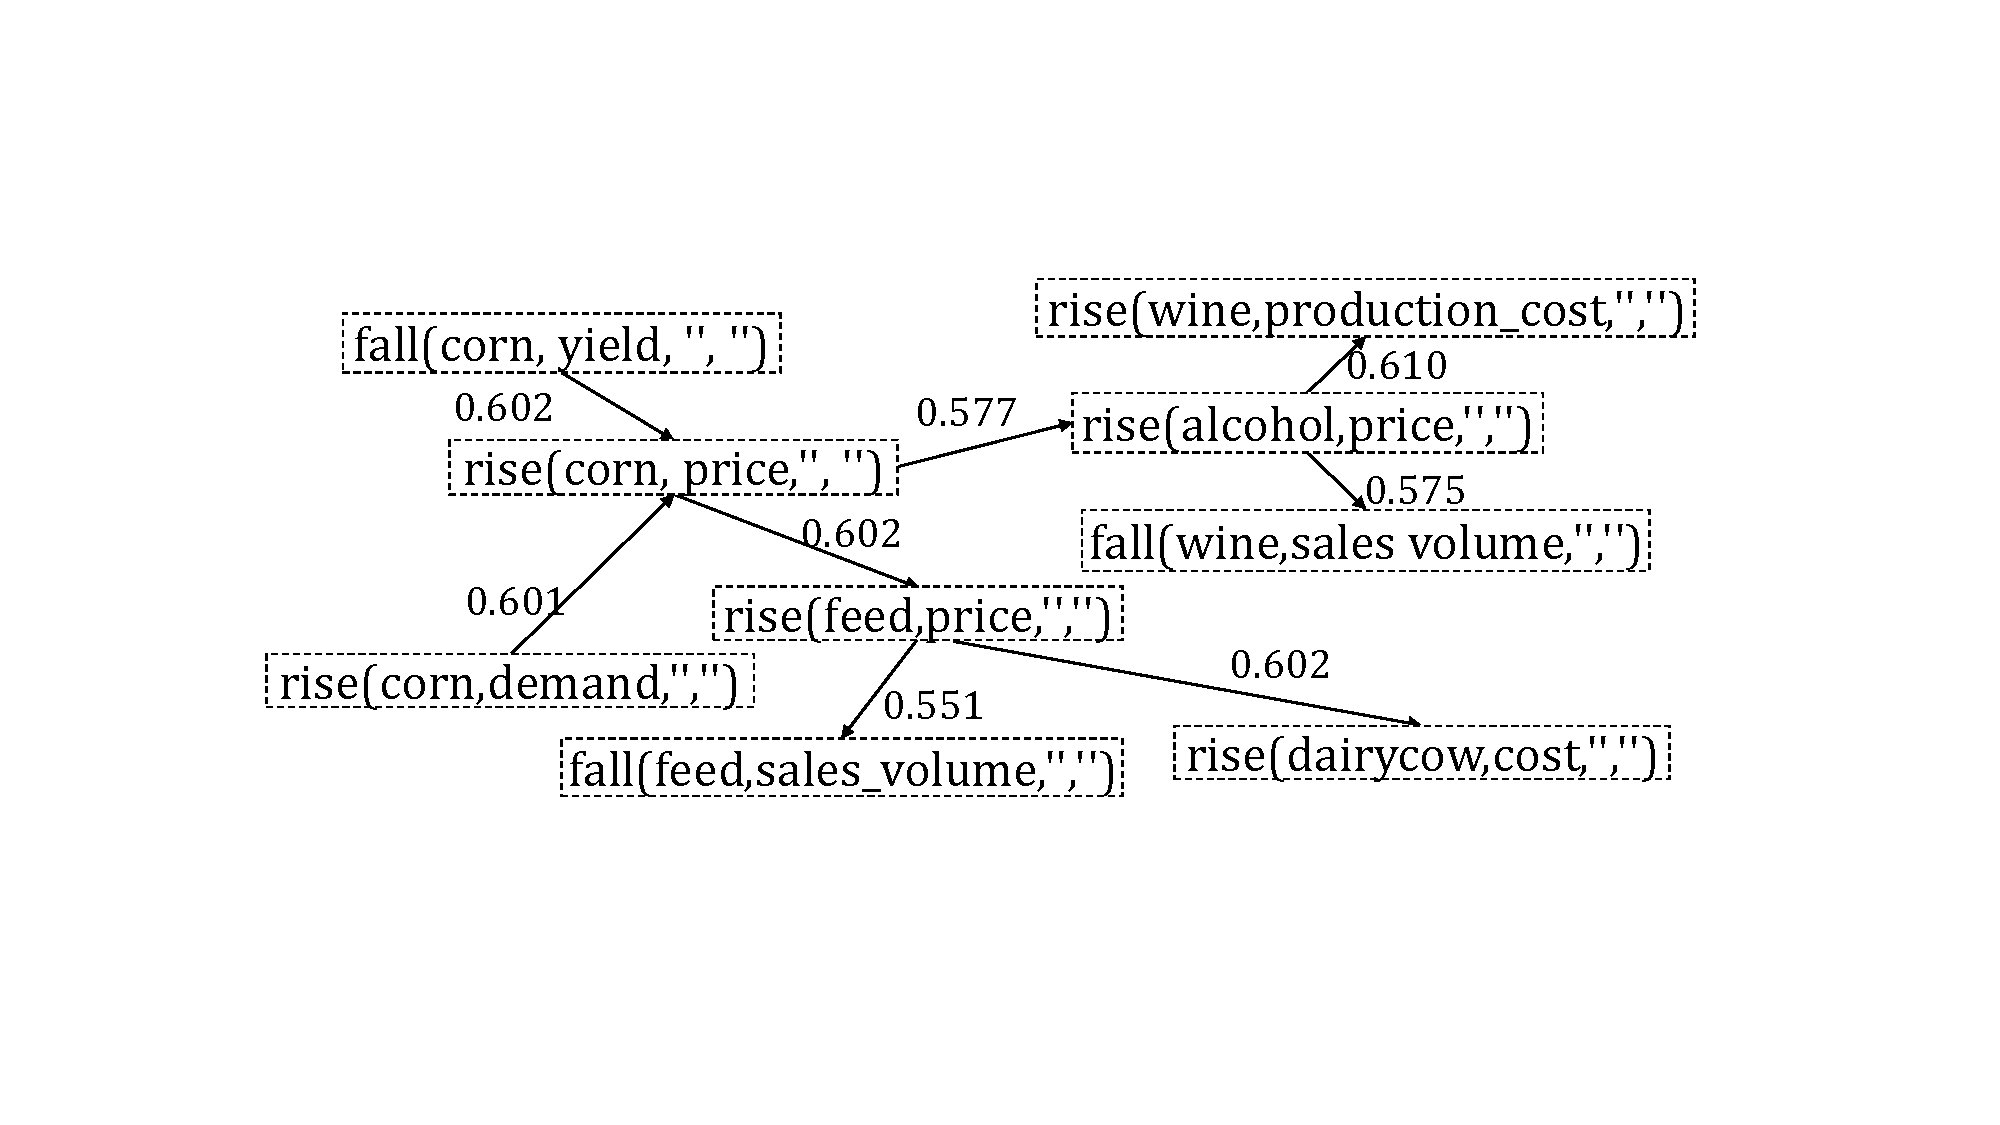
\includegraphics[width=0.9\columnwidth]{figures/event_graph}
\end{center}
\caption{Rule Instantiation. As space is limited, we only show the English version and omit the rules used in the reasoning process.}
\label{fig:rule_instantiation_graph}
\end{figure}

\section{An executable Example}
\label{sec:executable_example}
In this section, we demonstrate a tiny executable example to illustrate how to use the learned rules to do uncertain causal reasoning. 
The preliminary materials are a rule base, \zhpro, \zhcon, a financial instance lexicon, a Chinese synonym lexicon CiLin. 
To make it simple, here, we assume that the rule base only has only the rule (1).
The specific reasoning steps are as follows:
First, given a query sentence: ``Thailand suffered an earthquake attack". 
Second, extract the structured event: (`', Thailand, suffer, earthquake, attack), and convert it into the Prolog form `suffer(-, thailand, earthquake, attack, Es, 1, Cs)', where the variables, whose first letter is capitalized, are used to return the reasoning results. Sometimes, we can extract more than two events, then we repeat the reasoning processing multiple times. 
Third, search for the related rules and facts. We get the only rule and related facts: isA(thailand, country), isA(earthquake, disaster), atLocation(rice, thailand), isA(rice, product).
Fourth, convert them into standard Prolog code, shown in Listing \ref{lst:executable_example} from Line 1 to Line 12.
Last, input the converted query into SWI-Prolog shown in Listing \ref{lst:executable_example} from Line 14 to Line 19.
Thus, we can predict the price of rice will increase with confidence of 0.84 if Thailand suffered an earthquake attack.
Furthermore, if we search for these two related facts: isA(rubber, product), 
atLocation(rubber, thailand), we can also predict that the price of rubber will rise.
\begin{listing}[htbp]
\begin{minted}[xleftmargin=3em,linenos,breaklines]{Prolog}
# ~~~~~~~~~~test.pl~~~~~~~~~~
# Some factual triples
isA(thailand, country).
isA(earthquake, disaster).
isA(rice, product).
atLocation(rice, thailand).
# The threshold is 0.3
isconfident(X):-X > 0.3. 
# This is auxiliary code to let the engine know the predicate `rise'.
rise(_,_,_,_,[],_,[]).
# This is the rule.
suffer(-, X, Y, attack, Es, C, Cs):-rise(Z, price, -, -, EIs, CI, CIs), isA(X, country), isA(Y, disaster), isA(Z, product), atLocation(Z, X), is(CI, 0.84*C), isconfident(CI), append(EIs, [rise(Z, price, -, -)], Es), append(CIs, [0.84], Cs).

# ~~~~~~~~~~swipl test.pl~~~~~~~~~~
# swipl is the command of Swi-Prolog.
?- suffer(-, thailand, earthquake, attack, Es, 1, Cs).
Es=[rise( rice, price, -, -)],
Cs=[0.84].
?-
\end{minted}
\caption{an executable example with our rule.}
\label{lst:executable_example}
\end{listing}

%\begin{minted}{c}
%	int main() {
%		printf("hello, world");
%		return 0;
%	}
%\end{minted}
%`append' predicate in Line 12 is auxiliary code, which is helpful to run in Swi-Prolog.
%Fifth, query ``suffer(-, thailand, earthquake, attack, Es, 1, Cs)." in SWI-Prolog.
%Get predicted events with confidences:\\
%Es=[rise(rice, price, -, -)],\\
%Cs=[0.84];

%Thus, we can predict the price of rice will increase with confidence of 0.84 if Thailand suffered an earthquake attack.
%Furthermore, if we search for these two related facts: isA(rubber, product), atLocation(rubber, thailand), we can also predict that the price of rubber will rise.

\subsection{Downloading and Demo}
\zhpro, \zhcon and learned rules are available at URL.
We also build a demo to demonstrate the reasoning process at URL. 

%We also developed an application demo of futures prices change triggering that can monitor news from around the world in real time, find the news that may cause futures prices changes, and alert users. Visit URL.


%
%\subsection{Application: Futures Price Prediction}
%%\paragraph{Reasoning with Uncertainty}
%\begin{figure}[htbp]
%	\begin{center}
%		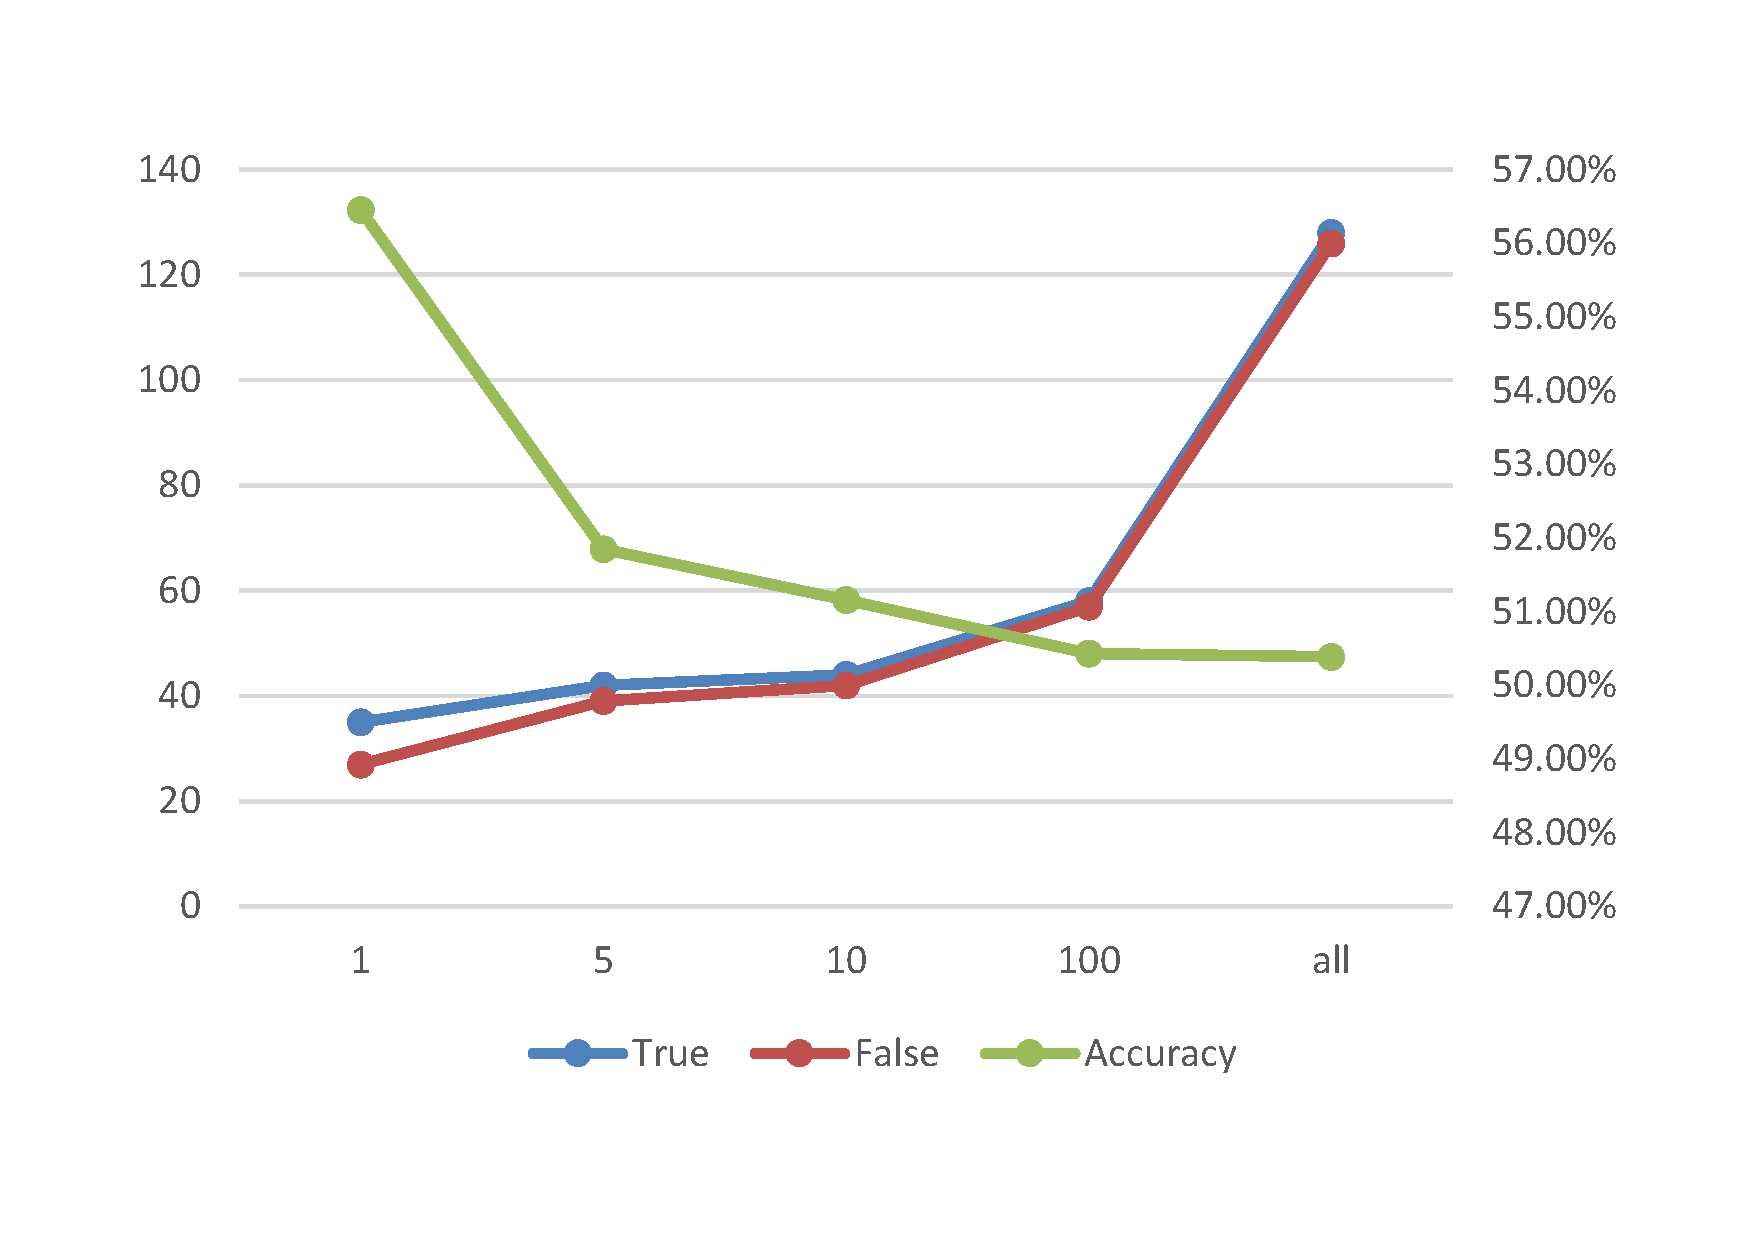
\includegraphics[width=0.9\columnwidth]{figures/rule_futures_prediction}
%	\end{center}
%	\caption{Futures Price Prediction.}
%	\label{fig:futures_price_prediction}
%\end{figure}
%We choose futures price prediction because the futures are common and concrete things existed in ConceptNet and Probase, such as corn, oil, etc.
%%\cite{Ding} is the state-of-the-art stock prediction model(EB\_CNN). We follow similar experimental settings. 
%We follow similar experimental settings in \cite{Ding}.
%From 2018/1/1 to 2018/11/2, we collect all the headlines and the price change of 15 futures as test data, which include \textbf{851} price change events (The price change of more than 1\% relative to the previous day is an event and we only focus on rise or fall events). 
%
%Baseline models: EB\_CNN model \cite{Ding}, the state of the art model in stock price prediction, uses a deep convolutional neural network to model both short-term and long-term influences of events on stock price movements, and the accuracy of futures prediction is \textbf{54.2\%}. Other models in \cite{Ding}, such as EB\_NN, WB\_CNN, and WB\_NN can achieve \textbf{53.0\%}, \textbf{53.2\%}, and \textbf{53.5\%}, respectively. These accuracies of futures prediction are lower than the accuracies of stock prediction shown in the paper.
%It may be because the factors affecting the futures price are far less than the stock price and the futures price is much more stable than the stock price, which makes useful training information about the futures less and further affects the accuracy of the models.
%
%Implementation: For each actual future price change event , we get the news headlines for the previous month before this event. 
%For each news headline, we extract the event, use Prolog to reason based on the rules and external knowledge bases, and get the top K inferred events sorted by the confidence.
%We may have m*K inferred events for this event, m is the number of events occurred in this month. 
%Here, we select the price change events(rise or fall) of the future in this actual future price change event from m*K events and calculate the weighted sum of their confidences(rise event weights 1 and fall event weights -1). If the sum value is positive, we predict this future price as a rise event, otherwise as a fall event. If get no related events changing the future's price, do not make prediction. We compare this prediction with the actual price change to evaluate the reasoning effect. 
%Figure \ref{fig:futures_price_prediction} shows the average prediction result. It shows the more predicted events inferred from the Prolog(by increasing K) we use, the lower the prediction accuracy is(from \textbf{56.5\%} to \textbf{50.4\%}), and the more futures events we can predict(from \textbf{62} to \textbf{254}). 
%
%\textbf{\textit{To sum up}}, our rule-based prediction approach can have a higher prediction accuracy (56.45\%) and better interpretation ability with a low recall rate, which is very practical in life.

%\begin{table}[htbp]
%	\caption{Baselines and Proposed Framework}
%	\begin{center}
%		\begin{tabular}{lll}\hline
%			& Acc & MCC \\\hline
%			WB-NN &  0.535 &     \\
%			WB-CNN&  0.532  &     \\
%			EB-NN &  0.530  &     \\
%			EB-CNN&  0.542   &     \\
%			Rule &     &    \\\hline
%		\end{tabular}
%		\label{tab:baselines_and_rule}
%	\end{center}
%\end{table}